\documentclass[a4paper,10pt]{article}
\usepackage[utf8]{inputenc}
\usepackage{graphicx}
\usepackage{hyperref}
\usepackage{subcaption}
\usepackage{todonotes}

%opening
\title{OpenSEA - Implementational Details and Experimental Results}
\author{Patrick Klampfl}

\begin{document}

\maketitle

\begin{abstract}
This document contains information about implementational details of the soft-error analysis tool \emph{OpenSEA} as well as first experimental results.
\end{abstract}

\section{Introduction}
Soft-errors are flipped components (like latches, gates) in logical circuits caused by cosmic radiation. It is possible to detect soft-errors by adding redundancy in the form of
additional components, called protection-logic. Whenever a soft-error happens, the special alarm output should be raised.

OpenSEA is a tool to analyze the quality of such a protection logic. It provides several algorithms to either detect vulnerabilities or false positives.
A component is vulnerable when a soft-error occurs without raising the alarm-output by the protection logic. Vulnerabilities are false negatives.
False positives, on the other hand, are situations where an alarm is raised gratuitously, meaning that no soft-error occurred.

This document talks about the specifications (formats, conventions) and about experimental results of OpenSEA as a reference implementation for the newly developed algorithms. 
For information about the command-line parameters, please read the \emph{readme.md} file or execute \texttt{./immortal-bin -h}.

\section{Format specifications}
\subsection{Input circuit}
The tool takes a circuit in AIGER \footnote{\url{http://fmv.jku.at/aiger/FORMAT.aiger}} file-format (version 20071012) with an included protection circuit as input (Figure \ref{circuit-in}). The last output has to be the 
special \emph{alarm}-output, which is \emph{true} whenever a bit flip is detected by the internal protection logic.

\begin{figure}[!htb]
\centering
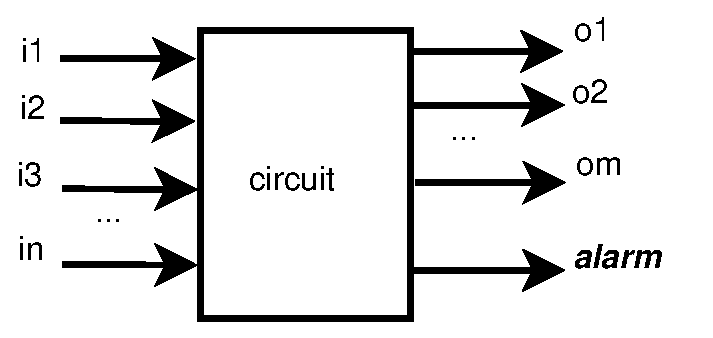
\includegraphics[scale = 0.48]{img/circuit-in.eps}
\centering \caption{The input circuit including the special \emph{alarm} output} 
\label{circuit-in}
\end{figure}

\subsection{Test Cases}
The input circuits are analyzed using so-called test cases, which provide the input-values for a given circuit.
Test cases are vectors of input vectors. An input vector defines the (usually concrete) input values of the circuit for one time step.
The number of input vectors can be arbitrary, however, the width of the input vectors has to match the number of inputs.

This is an example test-case for a two-inputs-circuit with a length of 3 time steps:
\begin{verbatim}
 1 0
 1 1
 0 0
\end{verbatim}


The previous test case consisted solely of concrete input values. Some algorithms/modes also allow to leave selected parts of the test-case undefined by using
a question mark instead of a concrete value.
In such a way, the sat-solver tries out all possible combinations of the unspecified input-values. Here is an example:
\begin{verbatim}
 1 0
 ? 1
 ? ?
\end{verbatim}

The input values for the initial time step are fixed in that example. The next time step  (\emph{ ? 1}) can be both (\emph{ 0 1}) or (\emph{ 1 1}). Finally, the last time step
can be set to all four possible 2-bit-combinations.


\subsection{Environment Models}  \label{environment}
In certain situations some output values might be irrelevant, for example when an output indicating that data on a bus is ready to be read is set to false.
If that is the case, then we do not care whether the output values on the data-bus are flipped or not. Such situations do not have to be reported as
vulnerabilities. On the contrary, a false-positive should still be reported if only irrelevant outputs are flipped.

The optional environment models can be used to specify under which circumstances an output is relevant. Like the original input circuit, they are 
encoded in the AIGER format as well. 

Environment circuits can use all inputs and all outputs of the original circuit as input. For the sake of implementational
simplicity, the number of inputs has to match: The input signals of the environment circuit are a concatenation of 
the inputs and outputs of the original circuits.
However, the environment model does not necessarily have to make use of all of the provided input signals.
The number of outputs must correspond to the original circuit, excluding the error-output. 
An environment output set to true indicates that the corresponding output in the original
circuit is relevant at this point in time.

Some algorithms allow to use test-cases with unspecified values, which can be set arbitrarily by the SAT-solver.
However, some input combinations may never occur in a practical mode of operation.
An optional output can be added to restrict the number of allowed input combinations. This additional output is
intended to be used as a formula talking about the input values which is true whenever the input combination is allowed.
With that, the SAT-solver sets the unspecified input values in such a way that that this output stays \emph{true} whenever possible.
If at some point it is not possible to set the open inputs accordingly, 
the algorithms won't find any further vulnerabilities/false-positives from this point forward.

\begin{figure}[!htb]
\centering
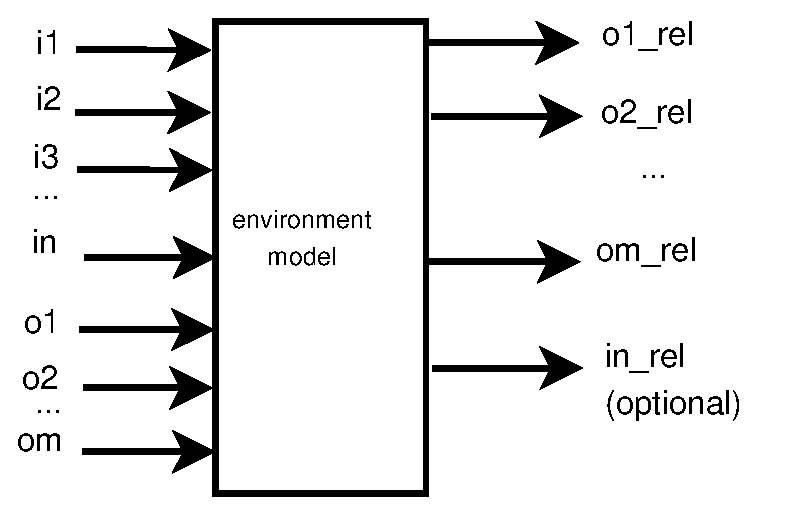
\includegraphics[scale = 0.48]{img/env.eps}
\centering \caption{An environment model defining relevance of outputs and optionally also allowed input combinations\emph{alarm} output} 
\label{env-img}
\end{figure}

\subsection{Output Format}
After analyzing the quality of the protection logic, the tool results in a list of definite problems (if any).

When searching for vulnerabilities, a list of vulnerable latches is provided. Optionally, a detailed error-trace can be generated
for each vulnerable latch consisting of the concrete input values for each time step, the point in time, at which the latch has to be flipped,
and the point in time, at which the error has an effect on the output values.

When searching for false positives, the tool generates a list of the superfluous alarms, each consisting of a flipped component $C$,
the point in time $j$ where it has been flipped, a point in time $k$ where the alarm was raised gratuitously, and a point in time $i+1$ where 
the state is the same as it would have been without flipping in step $j$. Recall that to be a false positive, the output values between $j$ and $i+1$ must not change.
If the test case contained free input variables, a input trace with the concrete input values to reproduce the error can be generated.
\newpage
\section{Algorithms and Modes} \label{algorithms}
The tool currently includes three distinct types of algorithms.
\begin{itemize}
 \item Simulation-Based-Algorithm (\texttt{SIM})
 \item Symbolic-Time-Analysis (\texttt{STA})
 \item Symbolic-Time-Location-Analysis (\texttt{STLA})
\end{itemize}
The tool implements modes to find vulnerabilities for all three types, but only for the latter two to find false positives

The Simulation-Based-Algorithm exhaustively searches for vulnerabilities. Due to its exhaustive nature, free input values do not scale very well. Each open input-value doubles the number of
test cases.

Symbolic-Time-Analysis is a SAT-solver based algorithm where the point in time of a bit-flip in a \emph{specific} latch is symbolic.

Symbolic-Time-Location-Analysis is similar to the previously mentioned algorithm - with one important difference: not just the point in time of a bit-flip, but also the latch to flip is symbolic and can therefore be chosen
by the SAT-solver. That means that compared to \texttt{STA} unrolling the transition relation only once suffices to check all latches for vulnerabilities.

All modes can be used with an optional environment model (\ref{environment}).

\subsection{Modes for Vulnerabilities}
{%
\newcommand{\mc}[3]{\multicolumn{#1}{#2}{#3}}
\begin{center}
\begin{tabular}{c|c|l}
Algorithm & Mode & \mc{1}{c}{Description}\\
\hline \hline
\texttt{SIM}  & 0 & only for concrete input values\\
              & 1 & capable of free inputs (currently at most 64)\\
\hline
\texttt{STA} & 0 & copy whole transition relation when unrolling\\
  & 1 & symbolically simulate transition relation \\
  & 2 & capable of free inputs\\
\hline  
\texttt{STLA} & 0 & standard mode\\
  & 1 & capable of free inputs
\end{tabular}
\end{center}
}%

\subsection{Modes for False Positives}
{%
\newcommand{\mc}[3]{\multicolumn{#1}{#2}{#3}}
\begin{center}
\begin{tabular}{c|c|l}
Algorithm & Mode & \mc{1}{c}{Description}\\
\hline \hline
FP & 0 & \texttt{STA} based\\
  & 1 & \texttt{STLA} based \\
  & 2 & \texttt{STA} based + capable of free inputs\\
  & 3 & \texttt{STLA} based + capable of free inputs
\end{tabular}
\end{center}
}%

\newpage
\section{Experimental Results}
Several publicly available circuits like the 
IWLS 2002 \footnote{\url{http://www.eecs.berkeley.edu/~alanmi/benchmarks/iwls2002/iwls_1.0.tar.gz}}
and IWLS 2005 \footnote{\url{http://www.eecs.berkeley.edu/~alanmi/benchmarks/}} benchmarks
were used to measure the performance of our implementation.

For this, we first converted the circuits into the AIGER format using ABC. Then, we added a generic protection logic to them which compares the parity sum
of the previous latch inputs and the current latch outputs. To generate partially vulnerable circuits, our simple AddParityTool allows to specify the percentage of latches to protect.

Note that all of the following charts within this chapter are cactus-plots with a logarithmic y-axis showing the execution time.
The x-axis shows the number of benchmarks that can be solved within this time limit.


\subsection{Comparison of Algorithms}
\emph{OpenSEA} implements several algorithms with several modes (Section \ref{algorithms}). Figure \ref{all_modes} shows the execution times for all modes that are capable of finding \emph{vulnerabilities}.
As an input, three random concrete test cases with a length of 15 time steps are used for each benchmark.

As can be seen, the simulation based algorithm is the fastest when using only fixed concrete input values as a test-case. However, this algorithm does not allow to use open input values.
Open inputs potentially reduce the necessary number or length of test-cases to find soft-errors and provide more flexibility to the user.

Making not just the point in time but also the latch to flip symbolic clearly leads to a significant speed-up (\texttt{STA} vs \texttt{STLA}).

All modes to a given type of algorithm perform similarly on this set of benchmarks, however, a slight performance decrease of the free-inputs-modes (\emph{sta2}, \emph{stla1}) can be noticed.


\begin{figure}[!htb]
\centering
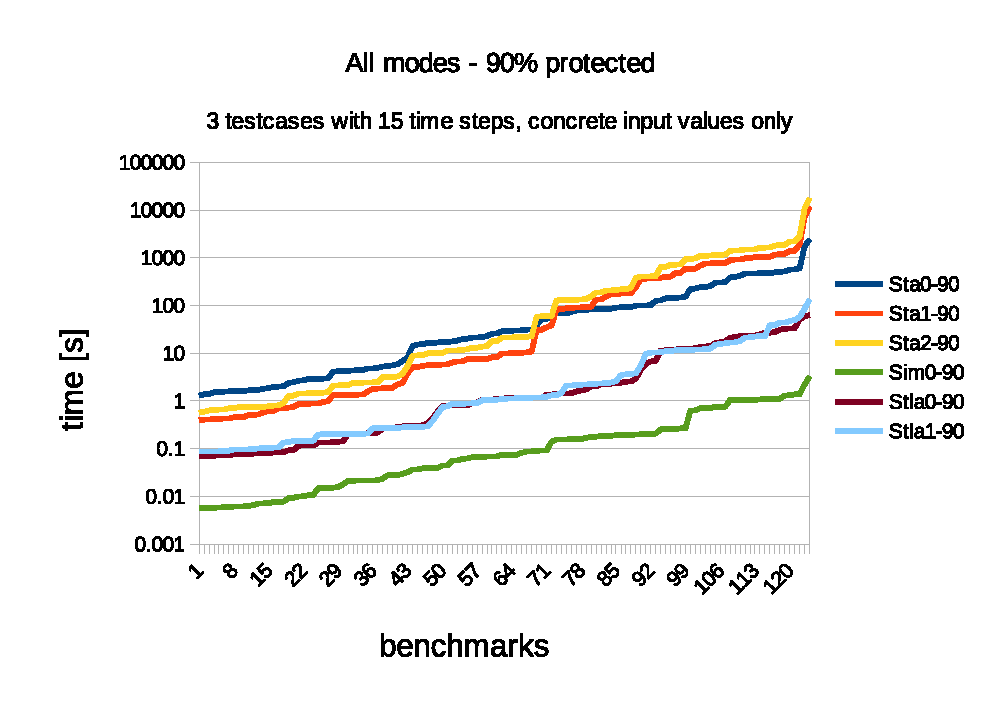
\includegraphics[scale = 0.5]{img/all_modes.eps}
\centering \caption{Execution times for all algorithms, using concrete input values}
\label{all_modes}
\end{figure}


\subsection{Length of the Test Cases}
The length of test cases (number of time steps) is one parameter that has an effect on the execution time. Longer test cases obviously result in a longer execution time.
Figure \ref{stla_input_length_chart} illustrates the influence of test case lengths: The \texttt{STLA} algorithm was executed with test case lengths of 15, 30, 60 and 100 time steps. 
No free input values were used, the randomly generated test-cases consisted solely of concrete input values (0 or 1).
The chart indicates an increase of execution time of roughly a half order of magnitude when doubling the test case length.

\begin{figure}[!htb]
\centering
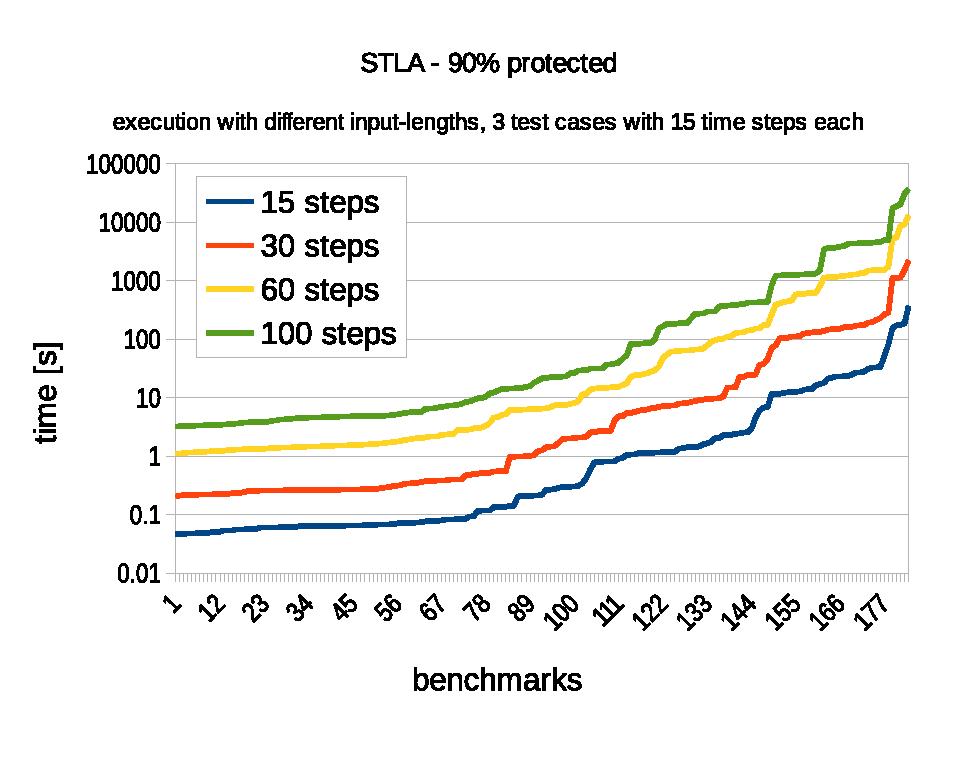
\includegraphics[scale = 0.6]{img/stla_input_length_chart.eps}
\centering \caption{\texttt{STLA 0} execution times for different test case lengths} 
\label{stla_input_length_chart}
\end{figure}

An increasing test case length in \texttt{SIM} only leads to a linearly growing run-time, as can be seen in Figure \ref{sim_input_length_chart}.

\begin{figure}[!htb]
\centering
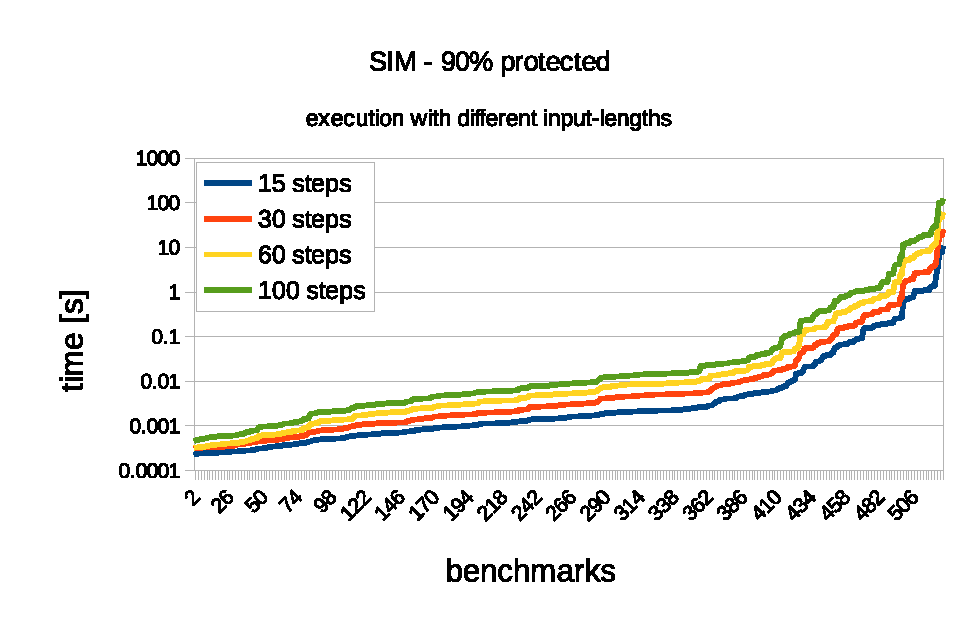
\includegraphics[scale = 0.6]{img/sim_input_length_chart.eps}
\centering \caption{\texttt{SIM 0} execution times for different test case lengths} 
\label{sim_input_length_chart}
\end{figure}

\subsection{Optimization: Unsatisfiable Cores}
The symbolic algorithms allow to compute unsatisfiable cores to reduce the number of variables while unrolling the transition relation. A reduced number of variables speeds up all following SAT-calls,
but the computation of the unsatisfiable cores are quite costly. Hence, it is necessary to find a meaningful interval instead of computing the cores for each time step.

The results for different core-computation-intervals with the \texttt{STLA} algorithm and test case lengths of 60 time steps can be seen in Figure \ref{uci-30ts}. Computing the unsatisfiable core all 5 time-steps on average almost cuts
the execution time in half (-45 \%).

In contrast, as Figure \ref{uci-15ts} indicates, the computation of unsatisfiable cores for shorter test cases (in this case 15 time steps) can decrease the performance.

\begin{figure}[!htb]
\centering
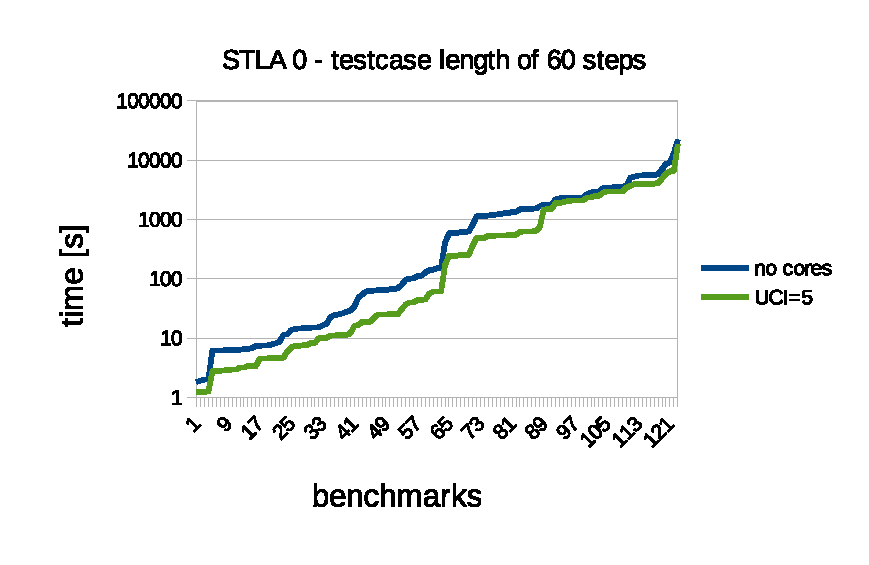
\includegraphics[scale = 0.57]{img/uci-60ts.eps}
\centering \caption{Computing an unsatisfiable core for longer test cases (here 60 time steps) increases the performance. The unsatisfiable core is computed at every 5th time step.} 
\label{uci-30ts}
\end{figure}

\begin{figure}[!htb]
\centering
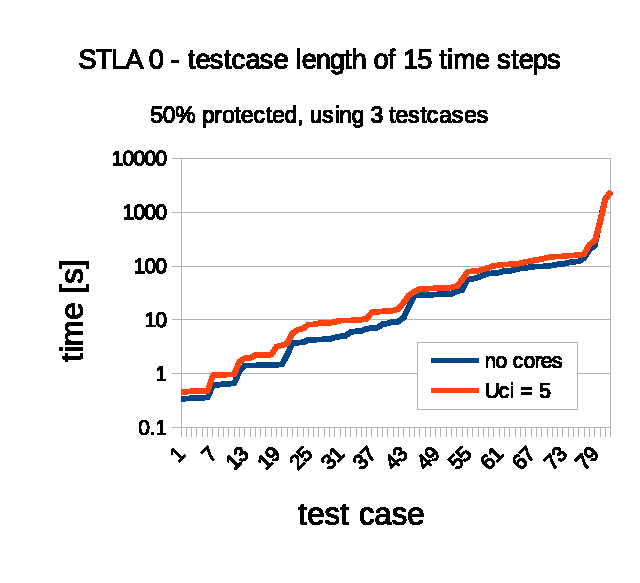
\includegraphics[scale = 0.57]{img/uci-15ts.eps}
\centering \caption{Computing an unsatisfiable core for shorter test cases (here 15 time steps) does not help} 
\label{uci-15ts}
\end{figure}

\subsection{Amount of Unspecified Input Values} \label{sec_free_inputs}
Using free input values in test cases allows to be more flexible, whereas concrete input values can be processed faster. In some cases however, free inputs might reduce the 
length or number of necessary test-cases.

In this section, we compare the run-time of our Symbolic-Time-Location-Analysis (\texttt{STLA}) using free input values with the naive simulation-based approach (\texttt{SIM}).
Recall, that each free input value in the worst case doubles the run-time when using a naive exhaustive approach.

\begin{figure}[!hbt]
\centering
  \begin{subfigure}[b]{0.95\linewidth}  \centering
    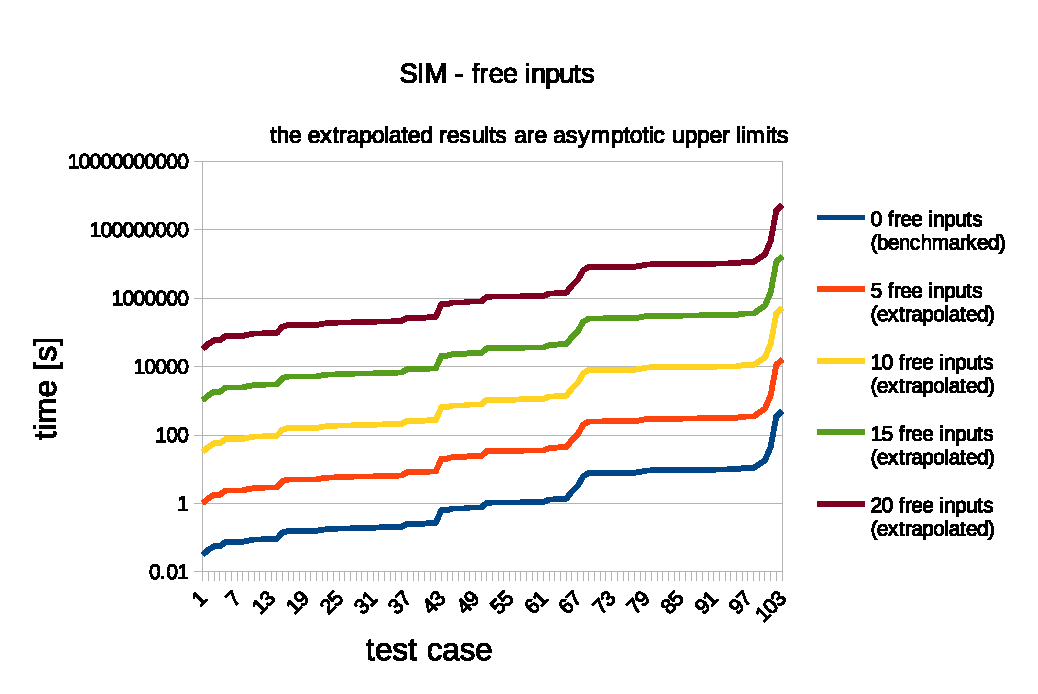
\includegraphics[width=\linewidth]{img/sim_free_inputs.eps}
    \caption{\texttt{SIM 1} benchmark results for free input values}
    \label{free_inputs_sim}
  \end{subfigure}
  \begin{subfigure}[b]{0.95\linewidth}  \centering
    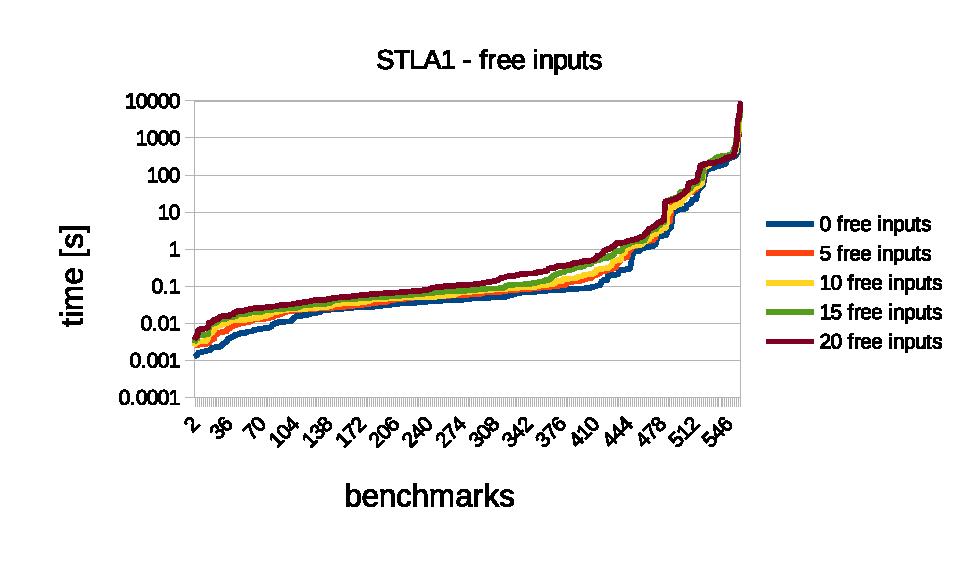
\includegraphics[width=\linewidth]{img/stla1_free_inputs.eps}
    \label{free_inputs_stla}
    \caption{\texttt{STLA 1}  benchmark results for free inputs}
  \end{subfigure}
  \caption{Using free input values scales significantly better for the \texttt{STLA 1} algorithm. Benchmarks are 90\% protected, 3 test cases, each of a lenght of 15 time steps. The free input values are located within the first time step(s). }
\label{fig_free_inputs}
\end{figure}
\todo{SIM benchmarks still running for more than 5 free inputs}

The chart in Figure \ref{fig_free_inputs} shows the effect of free input values on the execution time for both the \texttt{STLA} and the \texttt{SIM} algorithm.
\texttt{SIM} is the fastest algorithm when using only concrete inputs, as already mentioned in previous chapters. Just for concrete input values, converting a circuit to a CNF transition relation, unrolling it and then
performing SAT-solver calls seems to be impractical. However, that undoubtedly changes when free input values come into play. The \texttt{STLA} algorithm has the crucial ability to utilize the flexibility of SAT-solvers.
Because of that, the symbolic algorithm outperforms the simulation approach when it comes to scalability regarding free-input values. Both algorithms roughly have the same performance when using about 5 free input values.
For more free input values, \texttt{STLA} is the best choice, for fewer to none, \texttt{SIM} is faster.


It is arguable that optimizations for \texttt{SIM} could lead to a speed-up. For example because several input combinations
might lead to the same next-state. That certainly is a valid objection, it is however questionable if such an optimized simulation-based algorithm can be designed in such an elegant way as \texttt{STLA}. 
SAT-solvers, on the other hand, can cope with such problems very elegantly.


\subsection{Comparison with Model Checking}
In Section \ref{sec_free_inputs} we already discussed the influence of free input values. 
Model checking carries the idea of free inputs to an extreme: each input value for each time step (up to a specified time step bound) is a free input value. 
As a consequence, model checking is the most accurate, but also the computationally most expensive way to approach a soft error-analysis.

OpenSEA is capable of analyzing a circuit in a full model-checking mode, meaning that no concrete input values in a test case are used. 
Each mode that supports free inputs can be used for that.

Since most model checkers are highly optimized, this section shows results of a model checker (namely BLIMC) as well.
For this purpose, we wrote a small tool (\texttt{AlarmToMC}) which converts a circuit with protection logic to a model-checking problem, which again is a special type of circuit.
Model checkers typically take a circuit with exactly one output and try to find an input sequence which sets this error-output to true. 


Figure \ref{mc-chart} illustrates the enormous differences in execution time between a model-checking approach (using BLIMC and our \texttt{STLA 1}) and concrete input values only (\texttt{STLA 0}).


\begin{figure}[!htb]
\centering
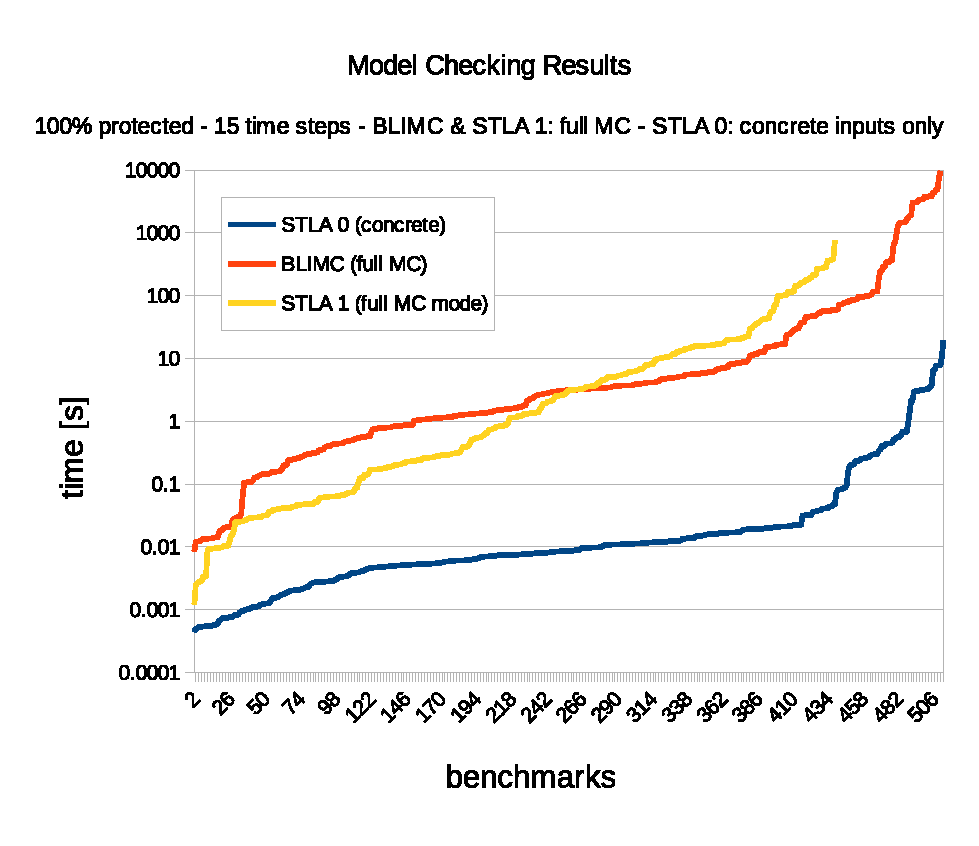
\includegraphics[scale = 0.64]{img/mc.eps}
\centering \caption{Both \texttt{BLIMC} model-checking for 15 time steps and \texttt{STLA 1} with 15 time steps of only free inputs try out all possible input combinations, 
whereas \texttt{STLA 0} uses only one concrete test case with a length of 15 time steps. } 
\label{mc-chart}
\end{figure}
\todo{STLA 1 and BLIMC benchmarks still running}

\newpage
\section{Conclusion}
Summing up the results, it can be concluded that symbolic algorithms like \texttt{STLA} scale better when it comes to free input values, whereas an analysis using concrete test-cases is carried out best with 
a simple simulation based approach (\texttt{SIM)} due to the lower computational overhead. In any case, concrete input values can be processed faster than free input values.
The results indicate that our \texttt{STLA} algorithm with free input values seems to be a good compromise between a simulation based- and a full model-checking approach.
The execution time for \texttt{SIM} grows only linearly for an increasing test case length, with \texttt{STLA}, it increases faster. Computing an unsatisfiable cores for longer test cases might be beneficial.

\end{document}
